\section*{ÔN TẬP KIỂM TRA CUỐI KÌ 1 - ĐỀ 06}
\setcounter{ex}{0}\setcounter{bt}{0}
\Opensolutionfile{ans}[ans/ansBTTeX6]

\begin{ex}%[Đoàn Minh Tân]%[0D4Y5-1]
Tam thức $f(x)=x^2-2x-3$ nhận giá trị dương khi và chỉ khi
\choice
{$x\in (-\infty;-3)\cup (-1;+\infty)$}
{\True $x\in (-\infty;-1)\cup (3;+\infty)$}
{$x\in (-1;3)$}
{$x\in (-3;1)$}
\loigiai{
Tam thức $f(x)=x^2-2x-3$ có $\Delta=16$, hai nghiệm $x_1=-1$, $x_2=3$ và hệ số $a=1>0$.\\
Bảng xét dấu của $f(x)$ như sau
\begin{center}

\begin{tikzpicture}
\tkzTabInit[nocadre=false, lgt=1.5, espcl=1.5]
{$x$ /0.6,$f(x)$ /0.6}
{$-\infty$,$-1$,$3$, $+\infty$}
\tkzTabLine{,+,0,-,0,+}
\end{tikzpicture}
\end{center}
Do đó $f(x)>0\Leftrightarrow x\in (-\infty;-1)\cup (3;+\infty)$.
}
\end{ex}

\begin{ex}%[Phạm Ánh Thư, sách giảng dạy Toán 10]%[0D4Y4-4]
Điểm $M\left(0;-3\right)$ thuộc miền nghiệm của hệ bất phương trình nào sau đây?
\choice
{\True $\heva{& 2x-y\leq 3\\ & 2x+5y\leq 12x+8}$}
{$\heva{& 2x-y>3\\ & 2x+5y\leq 12x+8}$}
{$\heva{& 2x-y>-3\\ & 2x+5y\geq 12x+8}$}
{$\heva{& 2x-y\leq -3\\ & 2x+5y\geq 12x+8}$}
\loigiai{
Thay toạ độ điểm $M\left(0;-3\right)$ vào hệ bất phương trình $\heva{& 2x-y\leq 3\\ & 2x+5y\leq 12x+8}$ ta có: $\heva{& 3\leq 3\\ & -15\leq 8}$ (đúng).
}

\end{ex}

\begin{ex}%[Trần Minh,Chuyển sách Tex - 10, 11 (dự án 3)]%[0H2Y3-1]
Tam giác $ ABC$ có $ AB=2$, $AC=1$ và $ \widehat{A}=60^\circ $. Tính độ dài cạnh $ BC$.
\choice
{$ BC=1$}
{$ BC=2$}
{$ BC=\sqrt{2}$}
{\True $ BC=\sqrt{3}$}
\loigiai
{Theo định lí hàm cô-sin, ta có\\
$ BC^2=AB^2+AC^2-2AB\cdot AC\cdot \cos{A}=2^2+1^2-2\cdot 2\cdot 1\cdot \cos 60^\circ =3\\
\Rightarrow BC=\sqrt{3}$.}
\end{ex}

\begin{ex}%[0D2Y3-1]
Hàm số nào dưới đây đồng biến trên $(3; 4)$?
\choice
{\True $y=\frac{1}{2} x^2-2 x+1$}
{$y=x^2-7 x+2$}
{$y=-3 x+1$}
{$y=-\frac{1}{2} x^2+x-1$}
\loigiai{Xét hàm số bậc hai $y=\dfrac{1}{2}x^2-2x+1$ có $a=\dfrac{1}{2}>0$ và $-\dfrac{b}{2a}=1$ có bảng biến thiên sau
\begin{center}
\begin{tikzpicture}
\draw[thick](-6,4)--(-6,0) (-7,2.8)--(3,2.8);
\path (-6.5,3.45)node{$x$} (-5.5,3.45)node[]{$-\infty$} (2.5,3.35)node[]{$+\infty$} (-1.45,3.45)node[]{$2$} (-6.55,1)node[]{$y$} (-5.5,2.4)node[]{$+\infty$} (-1.5,0.4)node[]{$-1$} (2.6,2.4)node[]{$+\infty$};
\draw[->] (-5.15,2.12)--(-2.03,0.44); \draw[->](-1.02,0.42)--(2.14,2.31);
\end{tikzpicture}
\end{center}
Vậy $y=\dfrac{1}{2}x^2-2x+1$ đồng biến trên $(3;4)$.
}
\end{ex}

\begin{ex}%[VanLo HoaTrung, du an tex hoa tai lieu 10]%[0D4Y4-1]
Cho bất phương trình $2x+3y \le 0$ $(1)$. Chọn khẳng định đúng trong các khẳng định sau
\choice
{Bất phương trình $(1)$ chỉ có một nghiệm duy nhất}
{Bất phương trình $(1)$ vô nghiệm}
{\True Bất phương trình $(1)$ luôn có vô số nghiệm}
{Bất phương trình  có tập nghiệm là $\mathbb{R}$}
\loigiai{
Bất phương trình $2x+3y-6\le0$. có miền nghiệm phần tô màu kể cả bờ là đường thẳng $2x+3y-6=0$.\\
Vậy bất phương trình vô số nghiệm.
}
\end{ex}

\begin{ex}%[0H1Y1-3]%[Dự án Tex hóa Tài Liệu 10 Mới - Dương Công Tạo]
Mệnh đề nào sau đây sai?
\choice
{\True $\vec{AA'}=\vec{0}$}
{$\vec{0}$ cùng hướng với mọi vectơ}
{$\left| \vec{AB} \right|>0$}
{$\vec{0}$ cùng phương với mọi vectơ}
\loigiai
{Ta có
\begin{itemize}
\item $\vec{AA}=\vec{0}\Rightarrow$ mệnh đề A sai.
\item $\vec{0}$ cùng phương và cùng hướng với mọi vectơ.
\item $\left| \vec{AB} \right|>0,\forall A,B$.
\end{itemize}
}
\end{ex}

\begin{ex}%[Trần Minh,Chuyển sách Tex - 10, 11 (dự án 3)]%[0H2Y3-1]
Tam giác $ ABC$ có $ AC=4$, $\widehat{BAC}=30^\circ$, $\widehat{ACB}=75^\circ $. Tính diện tích tam giác $ ABC$.
\choice
{$ S_{\Delta ABC}=8$}
{$ S_{\Delta ABC}=4\sqrt{3}$}
{\True $ S_{\Delta ABC}=4$}
{$ S_{\Delta ABC}=8\sqrt{3}$}
\loigiai
{Ta có $ \widehat{ABC}=180^\circ-(\widehat{BAC}+\widehat{ACB} )=75^\circ =\widehat{ACB}$.\\
Suy ra tam giác $ ABC$ cân tại $ A$ nên $ AB=AC=4$.\\
Diện tích tam giác $ ABC$ là $ S_{\Delta ABC}=\dfrac{1}{2}AB\cdot AC\sin \widehat{BAC}=4$.}
\end{ex}

\begin{ex}%[0D2Y3-3]
Trục đối xứng của parabol $y=-x^2+5x+3$ là đường thẳng có phương trình
\choice
{$x=\dfrac{5}{4}$}
{$x=-\dfrac{5}{2}$}
{$x=-\dfrac{5}{4}$}
{\True $x=\dfrac{5}{2}$}
\loigiai{
Trục đối xứng của parabol $y=a{x^2}+bx+c$ là đường thẳng $x=-\dfrac{b}{2a}$ .\\
Trục đối xứng của parabol $y=-x^2+5x+3$ là đường thẳng $x=\dfrac{5}{2}$.}
\end{ex}

\begin{ex} %[0D1Y2-2]
Trong các khẳng định sau. Hãy chọn khẳng định đúng?
\choice
{$\varnothing \subset \{\varnothing \}$}
{\True $\varnothing \subset \varnothing$}
{$\varnothing \in \varnothing$}
{$\{\varnothing\}\in \{\varnothing \}$}
\loigiai{}
\end{ex}

\begin{ex}%[Lê Quốc Dũng-Dự Án TEX TLDH5]%[0D1Y1-3]
Cho mệnh đề \lq\lq  $\forall x\in \mathbb{R},\, x^2-x+7 < 0$ \rq\rq . Mệnh đề nào là mệnh đề phủ định của mệnh đề trên?
\choice
{\True $\exists x\in \mathbb{R}$ mà $x^2-x+7\ge 0$}
{$\forall x\in \mathbb{R},\, x^2-x+7>0$}
{$\forall x\in \mathbb{R},\, x^2-x+7 < 0$}
{$\not {\exists } x\in \mathbb{R},\, x^2-x+7 < 0$}
\loigiai{
}
\end{ex}

\begin{ex}%[Lê Minh Thiện Anh, Dự án BG10-Lần2]%[0H2Y2-1]
\immini{Gọi $R$ là trung điểm cạnh $MN$ của tam giác đều $MNQ$. Xác định góc giữa $\overrightarrow{NR}$ và $\overrightarrow{NQ}$.
\choice
{$0^\circ$}
{\True $60^\circ$}
{$120^\circ$}
{$90^\circ$}
}
{
\begin{tikzpicture}[>=stealth,line join=round,line cap=round,font=\footnotesize,scale=1]
\path
(0,0)coordinate (Q)++(0:3)coordinate(N)++(120:1.5)coordinate(R)++(120:1.5)coordinate(M)
;
\draw (M)--(N)--(Q)--cycle;
\draw[->] (N)--(R);
\draw[->] (N)--(Q);
\foreach \x/\g in{M/90,N/0,R/45,Q/180}
\fill[black](\x)circle(1pt) ($(\x)+(\g:3mm)$)node{$\x$};
\end{tikzpicture}
}
\loigiai{
Góc giữa hai véc-tơ $\overrightarrow{NR}$ và $\overrightarrow{NQ}$ là $\widehat{QNR}=60^\circ$.
}
\end{ex}

\begin{ex}%[Trần Quốc, BG10-2022, Nhóm 9]%[0H1Y3-1]
Cho đoạn thẳng $AB$ và $M$ là một điểm trên đoạn $AB$ sao cho $AB=5AM$. Mệnh đề nào sau đây \textbf{sai}?
\choice
{$\overrightarrow{MA}=-\dfrac{1}{4}\overrightarrow{MB}$}
{$\overrightarrow{MB}=\dfrac{4}{5}\overrightarrow{AB}$}
{\True $\overrightarrow{MB}=-\dfrac{4}{5}\overrightarrow{AB}$}
{$\overrightarrow{AM}=\dfrac{1}{5}\overrightarrow{AB}$}
\loigiai{
\immini{
Dễ thấy rằng $\overrightarrow{MB}$ và $\overrightarrow{AB}$ là hai vectơ cùng hướng nên mệnh đề sai là $\overrightarrow{MB}=-\dfrac{4}{5}\overrightarrow{AB}$.
}
{\begin{tikzpicture}[scale=0.8,>=stealth, font=\footnotesize, line join=round, line cap=round]
\tkzDefPoints{0/0/A,5/0/B}
\draw (A)--(B);
\fill (0,0) node[above]{$A$} circle(1pt)
(1,0)node[above]{$M$}circle(1pt)
(2,0)circle(1pt)
(3,0)circle(1pt)
(4,0)circle(1pt)
(5,0)node[above]{$B$}circle(1pt);
\end{tikzpicture}}
}
\end{ex}

\begin{ex}%[Đoàn Minh Tân]%[0D4Y5-1]
Bảng xét dấu nào dưới đây là của tam thức $f(x)=-x^2+6x-9$?
\choice
{
\begin{tikzpicture}
\tkzTabInit[nocadre=false, lgt=1.5, espcl=1.5]
{$x$ /0.6,$f(x)$ /0.6}
{$-\infty$,$3$, $+\infty$}
\tkzTabLine{,+,0,-}
\end{tikzpicture}
}
{
\begin{tikzpicture}
\tkzTabInit[nocadre=false, lgt=1.5, espcl=1.5]
{$x$ /0.6,$f(x)$ /0.6}
{$-\infty$,$3$, $+\infty$}
\tkzTabLine{,-,0,+}
\end{tikzpicture}
}
{\True 
\begin{tikzpicture}
\tkzTabInit[nocadre=false, lgt=1.5, espcl=1.5]
{$x$ /0.6,$f(x)$ /0.6}
{$-\infty$,$3$, $+\infty$}
\tkzTabLine{,-,0,-}
\end{tikzpicture}
}
{
\begin{tikzpicture}
\tkzTabInit[nocadre=false, lgt=1.5, espcl=1.5]
{$x$ /0.6,$f(x)$ /0.6}
{$-\infty$,$3$, $+\infty$}
\tkzTabLine{,+,0,+}
\end{tikzpicture}
}
\loigiai{
Tam thức $f(x)=-x^2+6x-9$ có $\Delta=0$, nghiệm kép $x=3$ và hệ số $a=-1<0$ nên có bảng xét dấu như sau
\begin{center}

\begin{tikzpicture}
\tkzTabInit[nocadre=false, lgt=1.5, espcl=1.5]
{$x$ /0.6,$f(x)$ /0.6}
{$-\infty$,$3$, $+\infty$}
\tkzTabLine{,-,0,-}
\end{tikzpicture}
\end{center}
}
\end{ex}


\begin{ex}%[0D3B2-4]
Nghiệm của phương trình $\sqrt{x-1}=\left(\sqrt{3-x}\right)^2$ là
\choice
{$x=2;x=5$}
{\True $x=2$}
{$x=1;x=3$}
{$x=-1;x=-3$}
\loigiai{
Ta có
\allowdisplaybreaks
\begin{eqnarray*}
\sqrt{x-1}=\left(\sqrt{3-x}\right)^2	&\Rightarrow & \sqrt{x-1}=3-x\\
& \Rightarrow  & x-1=(3-x)^2 \\
& \Rightarrow & x^2-7x+10=0\\
&\Rightarrow & \hoac{&x=2\\&x=5}.
\end{eqnarray*}
Chỉ có nghiệm $x=2$ thỏa mãn phương trình ban đầu. \\
Vậy $S=\{2\}$.
}
\end{ex}

\begin{ex}%[0D2B1-3]
\immini{
Cho hàm số $y=f(x)$ có tập xác định là $[-3;3]$ và đồ thị của nó được biểu diễn bởi hình bên. Khẳng định nào dưới đây là đúng?
\choice
{Hàm số nghịch biến trên khoảng $(1;0)$}
{Hàm số nghịch biến trên khoảng $(0;3)$}
{\True Hàm số nghịch biến trên khoảng $(-1;1)$}
{Hàm số đồng biến trên khoảng $(-1;4)$}
}{
\begin{tikzpicture}
\draw[>=stealth,->] (-2.5,0) -- (3.5,0) node[above]{\scriptsize $x$};
\draw[>=stealth,->] (0,-1.5) -- (0,2.5) node[left]{\scriptsize $y$};
\draw (0,0) node[below left]{\scriptsize $O$};
\draw [thick] (-2,0)--(-1,1)--(1,-1)--(3,2);
\foreach \i in {-2,-1,1,3}
\draw (\i,0.03) -- (\i,-0.03);
\foreach \i in {-1,1,2}
\draw (0.03,\i) -- (-0.03,\i);
\foreach \i in {-2,-1,1,3}
\draw (\i,0) node[below]{\scriptsize $\i$};
\foreach \i in {-1,1,2}
\draw (0,\i) node[right]{\scriptsize $\i$};
\draw [dashed] (-1,0)|-(-1,1) (1,0)|-(0,-1);
\draw [dashed] (3,0)|-(0,2);
\end{tikzpicture}
}
\loigiai{Dựa vào đồ thị hàm số, ta có hàm số nghịch biến trên khoảng $(-1;1)$.}
\end{ex}

\begin{ex}%[0D3B2-4]
Số nghiệm của phương trình 	$\sqrt{x^2-3x-2}=\sqrt{x-3}$ là
\choice
{\True 1}
{0}
{2}
{3}
\loigiai{
\begin{eqnarray*} \sqrt{x^2-3x-2}=\sqrt{x-3}
&\Rightarrow& x^2-3x-2 = x-3\\
& \Rightarrow & x^2 -4x+1= 0\\
& \Rightarrow & \hoac{& x=2+\sqrt{3} \\& x=2-\sqrt{3}.}
\end{eqnarray*}
Chỉ có nghiệm $x=2+\sqrt{3}$ thỏa mãn phương trình ban đầu. \\ Vậy phương trình có 1 nghiệm và $S=\{2+\sqrt{3}\} $
}
\end{ex}

\begin{ex}%[Phan Anh]%[0D2B1-2]
Tìm tập xác định $\mathscr{D}$ của hàm số $y=\dfrac{2x-1}{(2x+1)(x-3)}$.
\choice
{$\mathscr{D}=(3;+\infty)$}
{\True $\mathscr{D}=\mathbb{R}\setminus\left\{-\dfrac{1}{2};3\right\}$}
{$\mathscr{D}=\left(-\dfrac{1}{2};+\infty\right)$}
{$\mathscr{D}=\mathbb{R}$}
\loigiai{
Hàm số xác định khi $\heva{
& 2x+1\ne 0 \\
& x-3\ne 0}\Leftrightarrow \heva{
& x\ne-\dfrac{1}{2} \\
& x\ne 3.}$\\
Vậy tập xác định của hàm số là $ \mathscr{D}=\mathbb{R}\setminus\left\{-\dfrac{1}{2};3\right\}$}
\end{ex}

\begin{ex}%[0D4B4-4]
Cặp số $(x;y)=(0;0)$ \textbf{không} là nghiệm của hệ bất phương trình nào trong các hệ bất phương trình sau?
\def\dotEX{}
\choice
{$\heva{& 2x-y<1 \\& x\ge 0 \\& y\le 1}$}
{\True $\heva{& 2x+y<1 \\& x\ge 0 \\& y<0}$}
{$\heva{& 2x-y<1 \\& x\ge 0 \\& y\ge 0}$}
{$\heva{& 2x+y<1 \\& x\le 0 \\& y<1}$}
\loigiai{Thay cặp số $(0;0)$ vào hệ bất phương trình $\heva{& 2x+y<1 \\& x\ge 0 \\& y<0}$, ta có
$\heva{& 2 \cdot 0+0=0<1 \\& 0 \ge 0 \\& 0<0}$ (sai).
}
\end{ex}

\begin{ex}%[0D4B4-1]
Miền nghiệm của bất phương trình $x+y \leq 2$ là phần không bị gạch sọc của hình vẽ nào trong các hình sau?
\choice
{
\begin{tikzpicture}[scale=1, font=\footnotesize, line join=round, line cap=round, >=stealth]
\def\xmin{-1}\def\xmax{3.0}\def\ymin{-1}\def\ymax{3.0}
\draw[->] (\xmin-0.2,0)--(\xmax+0.2,0) node[below] {\footnotesize $x$};
\draw[->] (0,\ymin-0.2)--(0,\ymax+0.2) node[right] {$y$};
\draw (0,0) node [below left] {$O$};
\foreach \x in {-1,1,2,3}\draw (\x,0.1)--(\x,-0.1) node [below] {\footnotesize $\x$};
\foreach \y in {-1,1,2,3}\draw (0.1,\y)--(-0.1,\y) node [left] {\footnotesize $\y$};
\clip (\xmin,\ymin) rectangle (\xmax,\ymax);
\draw[pattern = north west lines,smooth,samples=200,domain=\xmin:\xmax] plot (\x,{-1*(\x)+2});
\draw[pattern = north east lines,opacity=.3, line width = 1.2pt,draw=none] plot[domain=\xmin:\xmax] (\x, {-1*(\x)+2})--(-1,-1)--(-1,3)--cycle;
\end{tikzpicture}
}
{
\begin{tikzpicture}[scale=1, font=\footnotesize, line join=round, line cap=round, >=stealth]
\def\xmin{-3.0}\def\xmax{1}\def\ymin{-1}\def\ymax{3.0}
\draw[->] (\xmin-0.2,0)--(\xmax+0.2,0) node[below] {\footnotesize $x$};
\draw[->] (0,\ymin-0.2)--(0,\ymax+0.2) node[right] {$y$};
\draw (0,0) node [below left] {$O$};
\foreach \x in {-3,-2,-1,1}\draw (\x,0.1)--(\x,-0.1) node [below] {\footnotesize $\x$};
\foreach \y in {-1,1,2,3}\draw (0.1,\y)--(-0.1,\y) node [left] {\footnotesize $\y$};
\clip (\xmin,\ymin) rectangle (\xmax,\ymax);
\draw[pattern = north west lines,smooth,samples=200,domain=\xmin:\xmax] plot (\x,{1*(\x)+2});
\draw[pattern = north east lines,opacity=.3, line width = 1.2pt,draw=none] plot[domain=\xmin:\xmax] (\x, {1*(\x)+2})--(1,3)--(1,-1)--cycle;
\end{tikzpicture}
}
{\True
\begin{tikzpicture}[scale=1, font=\footnotesize, line join=round, line cap=round, >=stealth]
\def\xmin{-1}\def\xmax{3.0}\def\ymin{-1}\def\ymax{3.0}
\draw[->] (\xmin-0.2,0)--(\xmax+0.2,0) node[below] {\footnotesize $x$};
\draw[->] (0,\ymin-0.2)--(0,\ymax+0.2) node[right] {$y$};
\draw (0,0) node [below left] {$O$};
\foreach \x in {-1,1,2,3}\draw (\x,0.1)--(\x,-0.1) node [below] {\footnotesize $\x$};
\foreach \y in {-1,1,2,3}\draw (0.1,\y)--(-0.1,\y) node [left] {\footnotesize $\y$};
\clip (\xmin,\ymin) rectangle (\xmax,\ymax);
\draw[pattern = north west lines,smooth,samples=200,domain=\xmin:\xmax] plot (\x,{-1*(\x)+2});
\draw[pattern = north east lines,opacity=.3, line width = 1.2pt,draw=none] plot[domain=\xmin:\xmax] (\x, {-1*(\x)+2})--(3,3)--(-1,3)--cycle;
\end{tikzpicture}
}
{
\begin{tikzpicture}[scale=1, font=\footnotesize, line join=round, line cap=round, >=stealth]
\def\xmin{-3.0}\def\xmax{1}\def\ymin{-1}\def\ymax{3.0}
\draw[->] (\xmin-0.2,0)--(\xmax+0.2,0) node[below] {\footnotesize $x$};
\draw[->] (0,\ymin-0.2)--(0,\ymax+0.2) node[right] {$y$};
\draw (0,0) node [below left] {$O$};
\foreach \x in {-3,-2,-1,1}\draw (\x,0.1)--(\x,-0.1) node [below] {\footnotesize $\x$};
\foreach \y in {-1,1,2,3}\draw (0.1,\y)--(-0.1,\y) node [left] {\footnotesize $\y$};
\clip (\xmin,\ymin) rectangle (\xmax,\ymax);
\draw[pattern = north west lines,smooth,samples=200,domain=\xmin:\xmax] plot (\x,{1*(\x)+2});
\draw[pattern = north east lines,opacity=.3, line width = 1.2pt,draw=none] plot[domain=\xmin:\xmax] (\x, {1*(\x)+2})--(-3,3)--(-3,-1)--cycle;
\end{tikzpicture}
}
\loigiai{
\immini{
Biểu diễn miền nghiệm trên mặt phẳng $Oxy$:\\
- Vẽ đường thẳng $d: x+y=2$.\\
- Lấy điểm $O(0;0)$ thay tọa độ vào ta có $0+0 \leq 2$ đúng.\\
Vậy miền nghiệm bất phương trình là nửa mặt phẳng chứa điểm $O(0;0)$ và có bờ là đường thẳng $d$, kể cả đường thẳng $d$.
}{
\begin{tikzpicture}[scale=1, font=\footnotesize, line join=round, line cap=round, >=stealth]
\def\xmin{-1}\def\xmax{3.0}\def\ymin{-1}\def\ymax{3.0}
\draw[->] (\xmin-0.2,0)--(\xmax+0.2,0) node[below] {\footnotesize $x$};
\draw[->] (0,\ymin-0.2)--(0,\ymax+0.2) node[right] {$y$};
\draw (0,0) node [below left] {$O$};
\foreach \x in {-1,1,2,3}\draw (\x,0.1)--(\x,-0.1) node [below] {\footnotesize $\x$};
\foreach \y in {-1,1,2,3}\draw (0.1,\y)--(-0.1,\y) node [left] {\footnotesize $\y$};
\clip (\xmin,\ymin) rectangle (\xmax,\ymax);
\draw[pattern = north west lines,smooth,samples=200,domain=\xmin:\xmax] plot (\x,{-1*(\x)+2});
\draw[pattern = north east lines,opacity=.3, line width = 1.2pt,draw=none] plot[domain=\xmin:\xmax] (\x, {-1*(\x)+2})--(3,3)--(-1,3)--cycle;
\end{tikzpicture}
}
}
\end{ex}

\begin{ex}%[0D3B2-4]
Tổng các nghiệm của phương trình $\sqrt{3x^2 - 8x + 5} - \sqrt{11 - x}=0 $ là
\choice
{\True $\dfrac{7}{3}$}
{$\dfrac{11}{3}$}
{$-\dfrac{11}{3}$}
{$\dfrac{1}{3}$}
\loigiai{
\begin{eqnarray*} \text{Phương trình}
&\Rightarrow \sqrt{3x^2 - 8x + 5} = \sqrt{11 - x}\\
& \Rightarrow 3x^2 - 8x + 5 = 11 - x\\
& \Rightarrow 3x^2 - 7x -6 = 0\\
&\Rightarrow \hoac{&x =  3\\&x = -\dfrac{2}{3}.}\\
\end{eqnarray*}
Các nghiệm thỏa mãn phương trình ban đầu. \\
Nên phương trình có tập nghiệm $S = \left\lbrace3; -\dfrac{2}{3} \right\rbrace $.\\
Vậy tổng các nghiệm là $\dfrac{7}{3}$.
}
\end{ex}

\begin{ex}%[0H1B1-1]
 	Cho tứ giác $ ABCD $. Có thể xác định được bao nhiêu vectơ (khác $ \overrightarrow{0} $) có điểm đầu và điểm cuối là các điểm $ A $, $ B $, $ C $, $ D $?
 	\choice
 	{$ 4 $}
 	{$ 8 $}
 	{$ 10 $}
 	{\True $ 12 $}
 	\loigiai{Có thể xác định được 12 vectơ (khác $ \overrightarrow{0} $) có điểm đầu và điểm cuối là các điểm $ A $, $ B $, $ C $, $ D $ là các vectơ $ \overrightarrow{AB} $, $ \overrightarrow{AC} $, $ \overrightarrow{AD} $, $ \overrightarrow{BC} $, $ \overrightarrow{BD} $, $ \overrightarrow{CD} $ và các vectơ đối của chúng.
 	}
\end{ex}

\begin{ex}%[0H2B1-1]
Khẳng định nào sau đây \textbf{sai}?
\choice
{\True $\cos 75^\circ >\cos 50^\circ $}
{$\sin 80^\circ >\sin 50^\circ $}
{$\tan 45^\circ <\tan 60^\circ $}
{$\cos 30^\circ =\sin 60^\circ $}
\loigiai
{Trong khoảng từ $0^\circ $ đến $90^\circ $, khi giá trị của góc tăng thì giá trị cos tương ứng của góc đó giảm.}
\end{ex}

\begin{ex}%[0D4B5-2]
Tập nghiệm của bất phương trình $x^2 - 5x + 6 \leq 0$ là
\choice
{$(- \infty ; 2)$}
{$( - \infty ; 2 ] \cup [3; + \infty )$}
{$[3; + \infty )$}
{\True $[2;3]$}
\loigiai{
\[x^2 - 5x + 6 = 0 \Leftrightarrow \hoac{x &=2 \\ x &=3.}\]
Bảng xét dấu
\begin{center}

\begin{tikzpicture}
\tkzTabInit[nocadre=false, lgt=2, espcl=2.5]{$x$ /1,$f(x)$ /1}{$-\infty$,$2$,$3$,$+\infty$}
\tkzTabLine{,+,$0$,-,$0$,+,}
\end{tikzpicture}
\end{center}
}
\end{ex}

\begin{ex}%[0D2B3-1]
Xét tính đồng biến, nghịch biến của hàm số $f\left(x\right)=x^2-4x+5$ trên các khoảng $\left(-\infty;2\right)$ và $\left(2;+\infty\right)$. Khẳng định nào sau đây đúng?
\choice
{\True Hàm số nghịch biến trên $\left(-\infty;2\right)$, đồng biến trên $\left(2;\,+\infty\right)$}
{Hàm số nghịch biến trên các khoảng $\left(-\infty;\,2\right)$ và $\left(2;\,+\infty\right)$}
{Hàm số đồng biến trên $\left(-\infty;\,2\right)$, nghịch biến trên $\left(2;\,+\infty\right)$}
{Hàm số đồng biến trên các khoảng $\left(-\infty ;\,2\right)$ và $\left(2;\,+\infty\right)$}
\loigiai{
Tập xác định $\mathscr{D}=\mathbb{R}$.\\
Tọa độ đỉnh $I\left(2;\,1\right)$.\\
Bảng biến thiên:
\begin{center}

\begin{tikzpicture}
\tkzTabInit[nocadre=false,lgt=1.2,espcl=2.5,deltacl=0.6]
{$x$ /0.6, $y$ /2.5}
{$-\infty$,$2$,$+\infty$}
\tkzTabVar{+/$+\infty$,-/$1$,+/$+\infty$}
\end{tikzpicture}
\end{center}
Hàm số nghịch biến trên $\left(-\infty ;\,2\right)$, đồng biến trên $\left(2;\,+\infty\right)$.}
\end{ex}

\begin{ex}%[Dự án TLDH5-Nhóm Latex, Kiều Ngân]%[0D1B3-2]
Cho hai tập $A$, $B$ khác rỗng. Xác định tập hợp $\left(A\cup B\right)\setminus B$.
\choice
{\True $A\setminus B$}
{$B\setminus A$}
{$ A\cap B$}
{$\left(A\setminus B\right)\cup\left(B\setminus A\right)$}
\loigiai{
Ta có $x\in (A\cup B)\setminus B\Leftrightarrow\heva{&x\in A\cup B\\&x\notin B}\Leftrightarrow\heva{&\hoac{&x\in A\\&x\in B}\\&x\notin B}\Leftrightarrow\heva{&x\in A\\&x \notin B}\Leftrightarrow x\in A\setminus B$.\\
Suy ra $\left(A\cup B\right)\setminus B=A\setminus B$.
}
\end{ex}

\begin{ex}%[0H2B2-1]
 	Cho tam giác $ABC$ có cạnh $BC=6$ và đường cao $AH$. $H$ ở trên cạnh $BC$ sao cho $BH=2HC$. Tính $\overrightarrow{AB}\cdot \overrightarrow{BC}$.
 	\choice
 	{\True $-24$}
 	{$24$}
 	{$18$}
 	{$-18$}
 	\loigiai{
 		$\overrightarrow{AB}\cdot \overrightarrow{BC}=\left(\overrightarrow{AH}+\overrightarrow{HB}\right)\cdot \overrightarrow{BC}=\overrightarrow{AH}\cdot \overrightarrow{BC}+\overrightarrow{HB}\cdot \overrightarrow{BC}=\overrightarrow{HB}\cdot \overrightarrow{BC}=-24$.
 	}
 \end{ex}

\begin{ex}%[Huỳnh Đức Vũ, BG10-2022, Nhóm 9]%[0H1B3-2]
Cho tam giác $ABC$ và một điểm $M$ tùy ý. Hãy chọn hệ thức đúng.
\choice
{$2\overrightarrow{MA}+\overrightarrow{MB}-3\overrightarrow{MC}=\overrightarrow{AC}+2\overrightarrow{BC}$}
{$2\overrightarrow{MA}+\overrightarrow{MB}-3\overrightarrow{MC}=2\overrightarrow{AC}+\overrightarrow{BC}$}
{\True $2\overrightarrow{MA}+\overrightarrow{MB}-3\overrightarrow{MC}=2\overrightarrow{CA}+\overrightarrow{CB}$}
{$2\overrightarrow{MA}+\overrightarrow{MB}-3\overrightarrow{MC}=2\overrightarrow{CB}-\overrightarrow{CA}$}
\loigiai{
Ta có $2\overrightarrow{MA}+\overrightarrow{MB}-3\overrightarrow{MC}=2(\overrightarrow{MA}-\overrightarrow{MC})+\overrightarrow{MB}-\overrightarrow{MC}=2\overrightarrow{CA}+\overrightarrow{CB}$.
}
\end{ex}

\begin{ex}%[Trần Minh,Chuyển sách Tex - 10, 11 (dự án 3)]%[0H1B2-4]
Cho tam giác $ABC$ vuông cân đỉnh $A$, đường cao $AH$. Khẳng định nào sau đây \textbf{sai}?
\choice
{$\left| \overrightarrow{AH}+\overrightarrow{HB}\right|=\left| \overrightarrow{AH}+\overrightarrow{HC}\right|$}
{\True $\overrightarrow{AH}-\overrightarrow{AB}=\overrightarrow{AH}-\overrightarrow{AC}$}
{$\overrightarrow{BC}-\overrightarrow{BA}=\overrightarrow{HC}-\overrightarrow{HA}$}
{$\left| \overrightarrow{AH}\right|=\left| \overrightarrow{AB}-\overrightarrow{AH}\right|$}
\loigiai{
Do $\Delta ABC$ cân tại $A$, $AH$ là đường cao nên $H$ là trung điểm $BC$.\\
Ta có \\
$\heva{
& \left| \overrightarrow{AH}+\overrightarrow{HB}\right|=\left| \overrightarrow{AB}\right|=a \\
& \left| \overrightarrow{AH}+\overrightarrow{HC}\right|=\left| \overrightarrow{AC}\right|=a}$
$\Rightarrow \left| \overrightarrow{AH}+\overrightarrow{HB}\right|=\left| \overrightarrow{AH}+\overrightarrow{HC}\right|$.\\
$\heva{
& \overrightarrow{AH}-\overrightarrow{AB}=\overrightarrow{BH} \\
& \overrightarrow{AH}-\overrightarrow{AC}=\overrightarrow{CH}=-\overrightarrow{BH}}\Rightarrow \overrightarrow{AH}-\overrightarrow{AB}=\overrightarrow{AH}-\overrightarrow{AC}$  \textbf{sai}.\\
$\heva{
& \overrightarrow{BC}-\overrightarrow{BA}=\overrightarrow{AC} \\
& \overrightarrow{HC}-\overrightarrow{HA}=\overrightarrow{AC} \\}\Rightarrow \overrightarrow{BC}-\overrightarrow{BA}=\overrightarrow{HC}-\overrightarrow{HA}$.\\
$\left| \overrightarrow{AB}-\overrightarrow{AH}\right|=\left| \overrightarrow{HB}\right|=\left| \overrightarrow{AH}\right|$ (do $\Delta ABC$ vuông cân tại $A$).}
\end{ex}

\begin{ex}%[Trần Quốc, BG10-2022, Nhóm 9]%[0H1B3-1]
Gọi $ G $	 là trọng tâm của tam giác $ ABC $. Tập hợp điểm $ M $ trong mặt phẳng chứa tam giác $ ABC $ sao cho $ \left| \overrightarrow{MA} + \overrightarrow{MB}+ \overrightarrow{MC}\right|=6$ là
\choice
{đường tròn ngoại tiếp tam giác $ ABC $}
{đường tròn tâm $ G $ bán kính bằng $ 1 $}
{\True đường tròn tâm $ G $ bán kính bằng $ 2 $}
{đường tròn tâm $ G $ bán kính bằng $ 6 $}
\loigiai{
Ta có $G$ là trọng tâm $\triangle ABC$ nên $\overrightarrow{MA} + \overrightarrow{MB}+ \overrightarrow{MC}=3\overrightarrow{MG}$. \\
Do đó $\left|3\overrightarrow{MG}\right|=6 \Leftrightarrow MG=2$.\\
Vậy tập hợp điểm $ M $ là đường tròn tâm $ G $ bán kính bằng $ 2 $.
}
\end{ex}

\begin{ex}%[Võ Thị Thùy Trang - Tex hoa TLToan 10]13%[0D1B1-4]
Tìm mệnh đề đúng.
\choice
{Điều kiện cần và đủ để một số tự nhiên chia hết cho 15 là số đó chia hết cho 5}
{\True Điều kiện cần để $a+b$ là một số hữu tỉ là $a$ và $b$ đều là số hữu tỉ}
{Điều kiện đủ để có ít nhất một trong hai số $a, b$ là số dương là $a+b>0$}
{ Điều kiện cần và đủ để một tứ giác là hình chữ nhật là nó có hai đường chéo bằng nhau}
\loigiai
{ Điều kiện cần để $a+b$ là một số hữu tỉ là $a$ và $b$ đều là số hữu tỉ.
}
\end{ex}

\begin{ex}%[0H2B2-1]
 	Cho tứ giác lồi $ABCD$ có $AD=6$. Đặt $\overrightarrow{v}=\overrightarrow{AB}-\overrightarrow{DC}-\overrightarrow{CB}$. Tính $\overrightarrow{v} \cdot \overrightarrow{AD}$.
 	\choice
 	{$18$}
 	{$24$}
 	{\True $36$}
 	{$48$}
 	\loigiai{
 		$\overrightarrow{v}=\overrightarrow{AB}-\overrightarrow{DC}-\overrightarrow{CB}=\overrightarrow{AB}+\overrightarrow{CD}+\overrightarrow{BC}=\overrightarrow{AD}$ suy ra $\overrightarrow{v} \cdot \overrightarrow{AD}=A{D^2}=36$.
 	}
 \end{ex}

\begin{ex}%[0H1B1-1]
 	Cho tứ giác $ ABCD $. Có thể xác định được bao nhiêu vectơ (khác $ \overrightarrow{0} $) có điểm đầu và điểm cuối là các điểm $ A $, $ B $, $ C $, $ D $?
 	\choice
 	{$ 4 $}
 	{$ 8 $}
 	{$ 10 $}
 	{\True $ 12 $}
 	\loigiai{Có thể xác định được 12 vectơ (khác $ \overrightarrow{0} $) có điểm đầu và điểm cuối là các điểm $ A $, $ B $, $ C $, $ D $ là các vectơ $ \overrightarrow{AB} $, $ \overrightarrow{AC} $, $ \overrightarrow{AD} $, $ \overrightarrow{BC} $, $ \overrightarrow{BD} $, $ \overrightarrow{CD} $ và các vectơ đối của chúng.
 	}
\end{ex}

\begin{ex}%[Phan Anh]%[0D2B1-1]
Điểm nào sau đây thuộc đồ thị hàm số $y=\dfrac{1}{x-1}$?
\choice
{\True $M_1(2;1)$}
{$M_2(1;1)$}
{$M_3(2;0)$}
{$M_4(0;-2)$}
\loigiai{
Xét điểm $M_1$, thay $x=2$ và $y=1$
vào hàm số $y=\dfrac{1}{x-1}$ ta được $1=\dfrac{1}{2-1}$ ta thấy đúng nên nhận $M_1$.}
\end{ex}

\begin{ex}%[0H2B1-2]
Cho hai góc $\alpha $ và $\beta $ với $\alpha +\beta =180^\circ $. Tính giá trị của biểu thức \break $P=\cos \alpha \cos \beta -\sin \beta \sin \alpha $.
\choice
{$P=0$}
{$P=1$}
{\True $P=-1$}
{$P=2$}
\loigiai
{Hai góc $\alpha $ và $\beta $ bù nhau nên $\sin \alpha =\sin \beta $; $\cos \alpha =-\cos \beta $.\\
Do đó $P=\cos \alpha \cos \beta -\sin \beta \sin \alpha =-\cos^2\alpha -\sin ^2\alpha =-(\sin ^2\alpha +\cos^2\alpha )=-1$.}
\end{ex}


\begin{ex}%[Dương Quang - Tex hoa TLToan 10]%[0D1K3-3]
Lớp $10\mathrm{~A}$ có 45 học sinh. Trong đó có 12 học sinh có học lực giỏi, 30 học sinh có hạnh kiểm tốt, trong đó có 10 học sinh vừa lực giỏi vừa hạnh kiểm tốt. Học sinh được khen thưởng nếu được học lực giỏi hoặc hạnh kiểm tốt. Tìm số học sinh không được khen thưởng.
\choice
{\True $13$}
{ $35$ }
{ $23$}
{ $32$ }
\loigiai{
\begin{center}
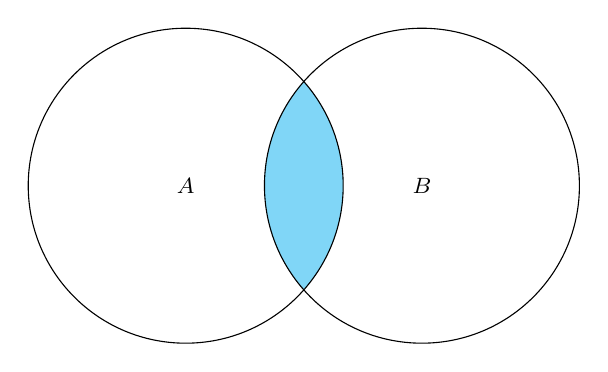
\begin{tikzpicture}[scale=1, font=\footnotesize, line join=round, line cap=round,>=stealth]
\coordinate (A) at (0,0);
\coordinate (B) at (3,0);
\begin{scope}
\clip(A) circle(2 cm);
\fill[cyan!50] (B) circle(2 cm);
\end{scope}
\draw (A) circle(2 cm) (B) circle(2 cm) (A)node{$A$} (B)node{$B$};
\end{tikzpicture}
\end{center}
Gọi $A, B$ lần lượt là tập hợp các học sinh giỏi và hạnh kiểm tốt của lớp $10\mathrm{A}$.\\
$\Rightarrow n(A)=12; n(B)=30; n(A\cap B)=10$.\\
Số học sinh được khen thưởng là \\
$n(A \cup B)=n(A)+n(B)-n(A\cap B)=12+30-10=32$.\\
Số học sinh không được khen thưởng là $45-32=13$ (học sinh).
}
\end{ex}
\Closesolutionfile{ans}
\begin{ex}[1,0 điểm]
Vẽ đồ thị hàm số $y=-x^2+3x+4$.
\end{ex}

\begin{ex}[0,5 điểm]%[Hoàng Thanh Phương, BG10-2022-Đợt 2, Nhóm 3]%[0D4B5-1]
Giải bất phương trình sau $4x^2+x-14>= 0$ bằng cách lập bảng xét dấu.
\loigiai{

}
\end{ex}

\begin{ex}[0,5 điểm]%[Phan Anh]%[Dự án giáo án 10]%[0H1B2-5]\begin{ex}%[0H1B3-1]%[Dự án TeX hoá tài liệu 10 mới, TVN-204]
Cho hình vuông $A B C D$ cạnh $a$, tâm $O$. Tính $|\overrightarrow{O B}+\overrightarrow{O C}|$.
% \choice
% {\True $|\overrightarrow{O B}+\overrightarrow{O C}|=a$}
% {$|\overrightarrow{O B}+\overrightarrow{O C}|=a \sqrt{2}$}
% {$|\overrightarrow{O B}+\overrightarrow{O C}|=\dfrac{a}{2}$}
% {$|\overrightarrow{O B}+\overrightarrow{O C}|=\dfrac{a \sqrt{2}}{2}$}
\loigiai{
\immini{
Gọi $I$ là trung điểm $BC$.\\
Khi đó $\overrightarrow{OB}+\overrightarrow{OC}=2\overrightarrow{OI}=\overrightarrow{AB}$.\\
Do đó $|\overrightarrow{O B}+\overrightarrow{OC}|=|\overrightarrow{AB}|=AB=a$.
}
{\begin{tikzpicture}[>=stealth,line join=round,line cap=round,font=\footnotesize,scale=.8]
\tikzset{declare function={a=2;b=2;goc=-90;}}
\coordinate (A) at (0:0);
\coordinate (D) at (0:a);
\coordinate (B) at (goc:b);
\coordinate (C) at ($(B)+(D)-(A)$);
\coordinate (O) at ($(A)!0.5!(C)$);
\coordinate (I) at ($(B)!0.5!(C)$);
\draw (A)--(B)--(C)--(D)--(A)--(C) (B)--(D) (O)--(I);
\foreach \d/\g in {A/135,B/200,C/-45,D/45,O/90,I/-90}\fill[black](\d) circle (.6pt)+(\g:.3)node[scale=.9]{$\d$};
\end{tikzpicture}
}
}
\end{ex}
\begin{ex}%[Nguyễn Tất Thu, BG10-2022]%[0H2K2-4]
Cho hai điểm $A$, $B$ cố định có độ dài bằng $a$.
Tìm tập hợp điểm $M$ sao cho $\overrightarrow{MA}\cdot \overrightarrow{MB}=MA^2$
\loigiai{
Ta có  \[\begin{aligned} \overrightarrow{MA}\cdot \overrightarrow{MB}=MA^2&\Leftrightarrow \overrightarrow{MA}\cdot \overrightarrow{MB}=\overrightarrow{MA}^2\\
&\Leftrightarrow \overrightarrow{MA}\cdot \left( \overrightarrow{MA}-\overrightarrow{MB} \right)=0\\ &\Leftrightarrow \overrightarrow{MA}\cdot \overrightarrow{BA}=0
\Leftrightarrow \overrightarrow{MA}\bot \overrightarrow{BA}.\end{aligned}\]
Vậy tập hợp điểm $M$ là đường thẳng vuông góc với đường thẳng $AB$ tại $A$.
}
\end{ex}

\begin{ex}[0,5 điểm]%[Đề kiểm tra HK2 môn Toán 10 trường THPT Nguyễn Thượng Hiền]%[Đoàn Minh Tân, 10EX-HK2-2223]%[0D4T5-6]
     Cho hình ngũ giác $ABCDE$ có $AB\perp BC$, $BC\perp DC$, $DC\perp DE$, $DE\perp AB$, $DE=AE=5$, $AB=9,BD=15$. Gọi $H$ là giao của $AB$ và $DE$ và đặt $HE=x$. Hãy thiết lập một phương trình để tính độ dài $x$, từ đó tính diện tích hình ngũ giác$ABCDE$.
\end{ex}